% !TEX root = ../../lectures.tex
\section{Cosmic ray spectrum from diffusive shock acceleration}

{\color{red}To be done}

%Let's explore the shock acceleration mechanism further through the formalism of a transport equation. We define our particle distribution function in the reference frame of the shock as:
%%
%\begin{equation}
%f = f(z, t, p)
%\end{equation}
%
%This function is defined such that the number density of particles is given by:
%%
%\begin{equation}
%n(z, t, p) dp = f(z, t, p) d^3 \mathbf{p} = f(z, t, p) 4 \pi p^2 dp
%\end{equation}
%
%The transport equation governing the distribution \( f \) is:
%%
%\begin{equation}
%\frac{\partial f}{\partial t} + u\frac{\partial f}{\partial z} - \frac{1}{3}\left(\frac{du}{dz}\right)p\frac{\partial f}{\partial p} = \frac{\partial}{\partial z}\left[D_{zz} \frac{\partial f}{\partial z}\right] + Q
%\end{equation}
%
%We pass now to characterise the \emph{injection term} \( Q(p) \). Without injection terms or a nonzero initial condition, the only solution to this transport equation is \( f(z, p, t) = 0 \) everywhere.
%
%It's important to remind that the shock is collisionless and possesses a small but finite thickness, comparable to the Larmor radius of the thermal particles forming the shock. For typical shock velocities of a few thousand kilometers per second, the Larmor radius is around \( r_{\rm L} \sim 10^8 \) cm, which, although small, is significant in astrophysical systems.
%%
%The gas in the downstream of the shock is thermalized, meaning its momentum distribution is Maxwellian. High-energy particles near the shock surface, which are part of this distribution, may have a Larmor radius large enough to cross the shock. Once they do, they enter the Fermi acceleration process, start gaining energy, and deviate from the Maxwellian distribution. This process constitutes the \emph{particle injection mechanism}. The likelihood of crossing the shock decreases with distance from the shock, as a larger Larmor radius would be necessary. This justifies the assumption that particles are injected at the shock.
%
%Consequently, we can represent the injection term as a delta-function in position:
%%
%\begin{equation}
%Q(z, t, p) \propto \delta(z) \delta(p - p_{\text{inj}})
%\end{equation}
%%
%where \( p_{\text{inj}} \) denotes the minimum momentum required for this process to occur.
%
%By introducing \( Q_0 \) to normalize the fraction of the particle flux crossing the shock per unit volume in phase space:
%%
%\begin{equation}
%\eta n_{\rm inj} u_1 = \int dz \, 4 \pi p^2 dp \, Q_0 \delta(z) \delta(p - p_{\text{inj}}) \rightarrow Q_0 = \eta \frac{n_{\rm inj} u_1}{4 \pi p^2_{\rm inj}}
%\end{equation}
%%
%hence, the transport equation becomes:
%%
%\begin{equation}
%\frac{\partial f}{\partial t} + u\frac{\partial f}{\partial z} - \frac{1}{3}\left(\frac{du}{dz}\right)p\frac{\partial f}{\partial p} = \frac{\partial}{\partial z}\left[D_{zz} \frac{\partial f}{\partial z}\right] + \delta(z) \delta(p-p_{\text{inj}})Q_0
%\end{equation}
%
%Assuming stationarity (\( \frac{\partial f}{\partial t} = 0 \)) and focusing on the upstream region where \( \frac{du}{dz} = 0 \), the equation becomes:
%%
%\begin{equation}
%u \frac{\partial f}{\partial z} - \frac{\partial}{\partial z} \left[D \frac{\partial f}{\partial z}\right] = 0 \rightarrow \frac{\partial}{\partial z}\left[uf - D \frac{\partial f}{\partial z}\right] = 0
%\end{equation}
%
%This implies that the sum of the advective and diffusive fluxes, \( uf - D\frac{\partial f}{\partial z} \), must be constant. Since it's unphysical to have accelerated particles at infinity in the upstream direction, the flux at \( z = +\infty \) is zero, and thus this constant value must also be zero:
%%
%\begin{equation}
%uf - D \frac{\partial f}{\partial z} = 0
%\end{equation}
%
%As an ansatz, we propose the following form for \( f \):
%%
%\begin{equation}
%f = f_0 \exp\left(\alpha z\right)
%\end{equation}
%
%Substituting this into the equation, we obtain \( \alpha = \frac{u_1}{D} \), leading to the upstream distribution function:
%%
%\begin{equation}
%f_{\rm u}(z, p) = f_0 \exp \left[ \frac{u_1 z}{D(p)} \right]
%\end{equation}
%
%Here, \( f_0 \) is the distribution function at the shock, serving as the boundary condition to solve the equation. The ratio \( \frac{D(p)}{u_1} \) is known as the \emph{typical diffusion length} of the plasma. This represents a balance point where the diffusion of particles away from the shock is counterbalanced by the plasma pushing them back towards the shock.
%
%In the downstream region, the only plausible stationary solution is to assume that the particle distribution function \( f_{\text{d}} = f_0 \) remains constant in space. This constancy is necessary because the particle density cannot diverge at downstream infinity (as this would be unphysical), and it cannot decrease either. If it did, diffusion and advection would concurrently remove particles from the downstream region, violating the stationary assumption.
%
%It's important to note that \( f \) is continuous across the shock. Unlike dynamic thermodynamic quantities, \( f \) is not a property of the plasma itself. The particles we're considering for acceleration have Larmor radii larger than the shock's thickness, meaning they do not \emph{feel} the discontinuity.
%
%To determine \( f_0 \), we integrate the transport equation across the shock:
%%
%\begin{equation}
%\lim_{\epsilon \rightarrow 0} \int_{-\epsilon}^{+\epsilon} \rightarrow 0 - \frac{1}{3}(u_2 - u_1) p \frac{\partial f_0}{\partial p} = D \left. \frac{\partial f}{\partial z} \right|_2 - D \left. \frac{\partial f}{\partial z} \right|_1 + Q_0 \delta (p-p_{\text{inj}})
%\end{equation}
%
%Here, the integral of \( \frac{\partial f}{\partial z} \) is zero since \( f \) is continuous across the shock. This leads to:
%
%\begin{equation}
%u_1f_0 - \frac{1}{3}(u_2-u_1)p\frac{\partial f_0}{\partial p} = Q_0\delta(p-p_{\text{inj}})
%\end{equation}
%
%For particles with \( p > p_{\text{inj}} \), we get:
%%
%\begin{equation}
%u_1f_0 = \frac{1}{3}(u_2-u_1)p\frac{\partial f_0}{\partial p}
%\end{equation}
%
%{\color{red}Rewriting this, we find:
%%
%\begin{equation}
%\begin{aligned}
%\frac{df_0}{f_0}&= -\frac{3u_1}{u_1-u_2}\frac{dp}{p}\\
%\log f_0 &= -\frac{3u_1}{u_1-u_2} \log p\\
%f_0(p)&= p^{-\frac{3u_1}{u_1-u_2}}= p^{-\frac{3u_1}{u_1-u_2}}\\
%f_0(p)&=\frac{3u_1}{u_1-u_2}\frac{N_{inj}\eta}{4\pi p^2_{inj}}\left( \frac{p}{p_{inj}}\right)^{-\frac{3r}{r-1}}\\
%f(p)&\propto p^{-\frac{3r}{r-1}}
%\end{aligned}
%\end{equation}
%
%\begin{equation}
%f_0(p) = \frac{3u_1}{u_1-u_2}\frac{N_{\text{inj}}\eta}{4\pi p^2_{\text{inj}}}\left( \frac{p}{p_{\text{inj}}}\right)^{-\frac{3r}{r-1}}
%\end{equation}
%
%\begin{equation}
%f(p) \propto p^{-\frac{3r}{r-1}}
%\end{equation}}
%
%This result confirms that:
%%
%\begin{equation}
%n(E) \sim p^2 f(p) \sim p^2 p^{-\frac{3r}{r-1}} \sim E^{-\frac{r+2}{r-1}} \rightarrow E^{-2}
%\end{equation}
%
%This relation holds for relativistic particles (\( E = p \)) and strong shocks (\( r = 4 \)). For non-relativistic particles (\( E = \frac{p^2}{2m} \)), the energy spectrum becomes\footnote{The number of particles with energy \( E$ is given by \( n(E)dE = 4\pi p^2 f_0(p) \left( \frac{dp}{dE} \right) dE \).}  \( n(E) \sim E^{-3/2} \).
%
%Thus, the spectrum of particles accelerated in diffusive shock acceleration is a power law in terms of momentum and a broken power law in terms of energy, with the break occurring at approximately the particle mass.
%
%\subsection{X-ray filaments}
%
%\begin{figure}[t!]
%\centering
%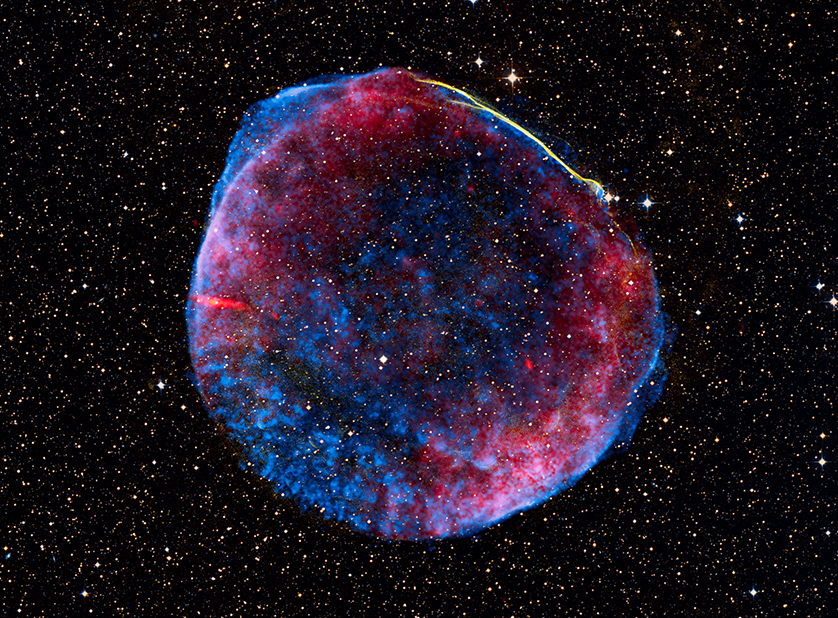
\includegraphics[width=0.65\textwidth]{sn1006c.jpg}
%\caption{Composite image of the SN 1006 supernova remnant. X-ray data from NASA’s Chandra X-ray Observatory are in blue.}
%\end{figure}
%
%X-ray synchrotron from SNR shocks first established for SN1006.
%
%Is related to loss-limited X-ray synchrotron emission.
%
%We equate the acceleration time with the synchrotron loss-time
%\[
%\tau_{\rm acc} = \frac{D}{u_s^2} \sim \tau_{\rm syn}
%\]
%%
%as \( \tau_{\rm syn} \propto E^{-1} B^{-2} \)
%
%follows that the max energy for which the two are the same
%%
%\[
%E \sim \frac{u_s^2}{B^2 D} 
%\]

